\documentclass[12pt]{report}
\usepackage[utf8]{inputenc}
\usepackage[english]{babel}
\usepackage{microtype}
\usepackage{libertine}
\usepackage{amsmath,amsthm}
\usepackage[varg]{newtxmath}\usepackage{setspace,graphicx,epstopdf}
\usepackage{marginnote,datetime,url,enumitem,subfigure,rotating}
\usepackage{todonotes}
\usepackage{xfrac}
\usepackage{graphicx}
\usepackage[open,openlevel=1]{bookmark}
\usepackage[tikz]{bclogo}
\usepackage{enumitem}

\setlength{\parindent}{0ex}
\setlength{\parskip}{1em}%Espacement des par

\setlist[itemize]{topsep=0pt}
\setlist[enumerate]{topsep=0pt}

\newtheorem{theorem}{Theorem}[chapter]
\newtheorem{definition}{Definition}[chapter]
\newtheorem{remark}{Remark}[chapter]
\newtheorem{axiom}{Axiom}[chapter]
\newtheorem{lemma}{Lemma}[chapter]
\newtheorem{proposition}{Proposition}[chapter]


\newcommand{\E}[1]{\operatorname{E}\left[#1\right]}
\newcommand{\V}[1]{\operatorname{Var}\left[#1\right]}
\newcommand{\cov}[1]{\operatorname{Cov}\left(#1\right)}
\newcommand{\Prob}[1]{\operatorname{Pr}\left[#1\right]}
\newcommand{\avg}[2]{\frac{#1}{#2} \sum_{i=#1}^{#2}}
\def\D{\mathrm{d}}

\newcommand{\smalltodo}[2][] {\todo[caption={#2}, size=\scriptsize,%
fancyline, #1]{\begin{spacing}{.5}#2\end{spacing}}}
\newcommand{\rhs}[2][]{\smalltodo[color=green!30,#1]{{\bf PS:} #2}}

\renewcommand\bcStyleTitre[1]{\textbf{#1}}

\begin{document}

\date{}
\title{\textbf{ECON7741 - Microeconomic Th. II}\\ \textit{Lecture Notes from Uzi Segal's course}}
\author{Paul Anthony Sarkis\\ Boston College} 
 
\maketitle

\tableofcontents

\chapter{Arrow's Impossibility Theorem}

\section{Social aggregation of preferences} 

Let our society consist in $n>1$ individuals with a common set of options X where $|X|\geq 3$. The set $X$ can be either finite or infinite. 

\begin{definition}[Individual Preference]
Each individual $i$ has a preference relation over $X$, denoted $\succeq_i$. This preference relation is assumed to be rational (complete and transitive).
\end{definition} 

\begin{definition}[Social Preference]
As a whole, we assume that society also has a preference relation over $X$, denoted $\succeq$.
\end{definition}

The question is what is the preference relation for the whole society? In other words, how can we find a society's preference relation?

\begin{definition}[Social aggregation process]
Let $\Omega$ be the set of all complete and transitive preference relations on $X$ (i.e. the set containing all possible orderings of all elements in $X$). A social aggregation process is a function defined on the set of all possible combinations of $n$ preference relations which returns one unique ordering. In mathematical terms: $$f:\Omega^n \to \Omega $$
\end{definition}

\begin{axiom}[Universal Domain]
A social aggregation process satisfies Arrow's axiom of Universal Domain if and only if it is defined on $\Omega^n$.
\end{axiom}

\subsection{Arrow's criteria for social aggregation} 

In our previously described society, let $a, b$ and $c$ be any options in $X$.

\begin{axiom}[Unanimity]
A social aggregation process satisfies Arrow's axiom of Unanimity if for all $i$, $$a \succ_i b \Rightarrow a \succ b$$ An alternative formulation would be that if for all $i$, $a \succeq_i b$ and $\exists j$ such that $a \succ_j b$, then $a \succeq b$.
\end{axiom}

\begin{axiom}[No-Dictatorship] 
A social aggregation process satisfies Arrow's axiom of Non-dictatorship if there does not exist an individual $i$ such that for all pairs $(a,b)$, the social aggregation process leads to the same result as $i$'s preference. 
$$\not\exists i: \forall \succeq_1,..., \succeq_{i-1},\succeq_{i+1},...,\succeq_n ; a \succ_i b \Rightarrow a \succ b $$
\end{axiom} 

\begin{axiom}[Transitivity]
A social aggregation process satisfies Arrow's axiom of Transitivity if for any $a,b,c\in X$, $$a \succeq b \text{ and } b \succeq c \Rightarrow a \succeq c$$
\end{axiom} 

\begin{axiom}[Independence of Irrelevant Alternatives] 
A social aggregation process satisfies Arrow's axiom of IIA if the social preference $\succeq$ between any $(a,b) \in X^2$ depends on individual preferences $\succeq_i$ over $(a,b)$

Formally, for any two social combination of preferences $\succeq_1,...,\succeq_n$ and $\succeq'_1,...,\succeq'_n$: $$ a \succeq_i b \Leftrightarrow a \succeq'_i b \Rightarrow a \succeq b \Leftrightarrow a \succeq' b $$
\end{axiom}

\subsection{The Majority Rule and Arrow's criteria} 

\begin{definition}[Majority Rule]
The majority rule is a social aggregation process that stipulates that, $a \succeq b$ if and only if the number of people who strictly prefer $a$ to $b$ is not smaller than the number of people who strictly prefer $b$ to $a$. That is, $$ a \succeq b \Leftrightarrow |{i:a\succ_i b}|\geq|{i:b\succ_i a}| $$
\end{definition}

\begin{remark}
Let $n$ be equal to 3 and $X = \{a, b, c\}$. There exists a combination of preferences such that a majority rule would violate transitivity.
\end{remark}
\begin{proof}
Let the three individuals have preferences such that:\begin{itemize}
\item[\textbf{P1:}] $a\succ_1 b \succ_1 c$
\item[\textbf{P2:}] $b\succ_2 c \succ_2 a$
\item[\textbf{P3:}] $c\succ_3 a \succ_3 b$
\end{itemize}
A majority rule would imply that $a\succ b, b\succ c$ and $c\succ a$. This is a violation of Arrow's axiom of transitivity.
\end{proof}

\section{Arrow's impossibility theorem}

\begin{theorem}[Arrow's Impossibility Theorem]
In a setting where there are at least 3 social options (the size of $X$ is greater than 2) there is no social ranking rule satisfying all five Arrow's axioms.
\end{theorem}

Before diving into the proof, we will require a few steps.

\begin{definition}[Extreme outcomes]
An outcome $b$ is defined as extreme in $\succeq$ if for any $a$ we have that $b\succeq a$ or $a\succeq b$.
\end{definition} 

\begin{lemma}
If for all $i$, $b$ is an extreme in $\succeq_i$, then it is also an extreme in $\succeq$.
\end{lemma}
\begin{proof}
Suppose b was not extreme in $\succeq$, then there exists two options $a$ and $c$ such that $a\succ b \succ c$, while everyone has one of those four rankings:\begin{itemize}
\item $b\succeq_i a \succeq_i c$
\item $b\succeq_i c \succeq_i a$
\item $a\succeq_i c \succeq_i b$
\item $c\succeq_i a \succeq_i b$
\end{itemize}
If we change all these preferences such that $c\succ_i a$ for all $i$. By IIA, the social ranking of $b$ compared to $a$ or $c$ does not change, therefore $a\succ b \succ c$. However, now by unanimity, it must be that $c\succ a$, therefore violating the transitivity rule.
\end{proof}

\begin{proof}[Arrow's Impossibility Theorem]
Now consider $n$ people subject to $k$ choices and where everyone agrees that $b$ is the worst outcome, ranking it last in the choices. In a process of $n$ steps, replace $b$ from last to first choice for one person at a time. We know that at step 0, $b$ is socially ranked last by unanimity; at time $n$, $b$ would be the best choice for society for the same reason. Moreover, by lemma 1, since every player chose $b$ as an extreme, $b$ was an extreme in $\succeq$ throughout the whole process: there must have been an individual for whom changing his decision changed the social ranking. 

We will show that this person, denoted by $i^*$, is the dictator.

Now we try to prove that this person dictates the social ranking for any other preference setting.

Define a profile where every individual up until $i^* -1$ changes their preferences to $\succeq'_i$, call it profile I. In this profile $a\succ b$ (the dictator has not changed yet).

Define another profile, call it profile II where the dictator has also changed his preferences to $\succeq'_i$. In this profile, $b\succ c$.

Let $a,c\neq b$ such that $a \succ_{i^*} c$ and any other relation for other individuals. 

Finally, consider a profile III where:\begin{itemize}
\item For all $i\neq i^*$, the preferences b/w $a$ and $c$ are the same as in the arbitrary profile defined above (not I nor II).
\item For the dictator $a \succ_{i^*} b \succ_{i^*} c$
\item For $i<i^*$, $b$ is the best outcome.
\item For $i>i^*$, $b$ is the worst outcome.
\end{itemize}

By IIA, the social preference between $a$ and $c$ must be the same in profile III and the arbitrary profile (only $b$ was different in profile III).

Moreover, the preferences between $a$ and $b$ are the same in profile I and III. Because profile I implies $a\succ b$, it should be the same in profile III.

In a similar manner, profile III and profile II share the same preferences for $b$ over $c$, which is that $b\succ c$.

Therefore, by transitivity, we must have that $a\succ b\succ c$ in profile III and the arbitrary profile, the same preferences as the dictator's.
\end{proof}

\section{Extensions of Arrow's impossibility theorem}

\subsection{Which axiom should go?} 

We proved that a social aggregation cannot follow all of Arrow's rules. Therefore, we need to let go of at least one, but which one?

\textbf{Universal Domain:} this rule might seem untouchable because it basically says, every type of preferences should be included in the process. However, we can imagine some types of preference that might not be desirable in a society or that might not make sense in a logical point of view.

\textbf{Unanimity:} again, this rule might be too anchored in our culture to judge it unnecessary but you might think about what it excludes. For example, future and past generations are excluded from this rule.

\textbf{Transitivity:}

\textbf{IIA:} There can be a real debate on whether other choices should affect the social aggregation for two specific choices.

\textbf{No dictatorship:}

\subsection{Restricting the type of preferences}

\begin{definition}[Single-peaked Preferences]
Let $X\subseteq\mathbb{R}$ such that all options in $X$ can be ordered numerically. A preference relation $\succeq$ is called single-peaked if there exists an $a^*$ such that,\begin{enumerate}
\item For any $b,c\in X$ satisfying $a^*>b>c$, we have $a^*\succeq b\succeq c$
\item For any $d,e\in X$ satisfying $a^*<d<e$, we have $a^*\succeq d\succeq e$
\end{enumerate}
\end{definition}

\begin{figure}[ht!]
\centering
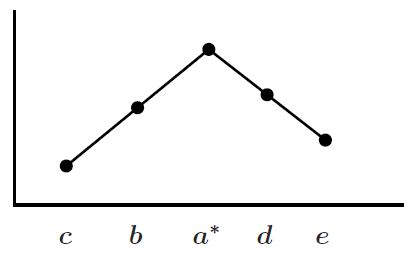
\includegraphics[scale=0.6]{images/sppref}
\caption{Single-peaked preferences over $\mathbb{R}$}
\end{figure}

\begin{theorem}[Majority rule under single-peaked preference]
If we restrict the domain of the majority rule process only to preferences satisfying single-peakedness, then the majority rule will satisfy all Arrow's axioms except Universal Domain.
\end{theorem}

\begin{proof}
\textbf{(Unanimity):} Nothing changes here, if for all $i$, $a\succeq_i b$, then the majority rule implies $a\succeq b$.

\textbf{(Transitivity):} Consider the policies $a>b>c$. Denote as $\alpha$ the number of people for which $a \succ_i b$, $\beta$ the number of people for which $b \succ_i c$ and $\gamma$ the number of people for which $a \succ_i c$. If $a\succ_i b$, then by single-peakedness we also have $b \succ_i c$ and $a\succ_i c$. Hence, $\alpha \leq \beta, \gamma$. If $c\succ_i b$, then by single-peakedness $c \succ_i a$ and $b \succ_i a$. Hence $n - \beta \leq n - \gamma \Leftrightarrow \beta \geq \gamma$ and $n - \beta \leq n - \alpha \Leftrightarrow \beta \geq \alpha$. Now,\begin{itemize}
\item if $a \succ b$, then $\alpha > n - \alpha$, and since $\beta, \gamma \geq \alpha$, we also have $\beta > n - \beta \Rightarrow b \succ c$ and $\gamma > n - \gamma \Rightarrow a \succ c$: transitivity is satisfied.
\item if $c\succ b$, then $n - \beta > \beta$, and since $\beta \geq \alpha, \gamma$, we also have $c\succ a$ and $b \succ a$: no violation of transitivity.
\item if nothing from above is satisfied, then $b\succ a$ and $b\succ c$: transitivity is not in danger.
\end{itemize}

\textbf{(IIA):} By the definition of a majority rule, a choice between $a$ and $b$ depends only on individual preferences over these choices.

\textbf{(No-dictatorship):} As a dictator cannot rule over a majority. This is also satisfied.
\end{proof}

\subsection{Liberalism and Sen's impossibility theorem} 

Economists proposed to replace the IIA by another objective for social aggregation: liberalism.

\begin{axiom}[Liberalism] 
A social aggregation process satisfies Sen's axiom of Liberalism if, for each individual $i$, there exists at least one pair of alternatives $a,b\in X$ such that $a\succeq_i b \Rightarrow a \succeq b$ and $b\succeq_i a \Rightarrow b \succeq a$.
\end{axiom} 
In words, this rule implies that every individual in society has at least a bit of dictatorial power, in turn reducing the likelihood of there being a unique dictator for every choice.

\begin{theorem}[Sen's Impossibility Theorem]
In a setting where there are at least 3 social options (the size of $X$ is greater than 2) there is no social ranking rule satisfying all of Arrow's axioms where IIA has been replaced by Liberalism.
\end{theorem}

\begin{proof} 
Let two individuals rank three options about a book "Lady Chatterley's Lover". Either no ones reads it ($a$), only person 1 reads it ($b$) or only person 2 reads it ($c$). Now suppose that for individual 1: $a \succ_1 b \succ_1 c$, whereas for individual 2: $b \succ_2 c \succ_2 a$. \begin{itemize}
\item[$(a,b)$:] Since this choice affects person 1 only, his decision should matter and by liberalism $a\succeq_1 b \Rightarrow a \succeq b$.
\item[$(a,c)$:] Since this choice affects person 2 only, his decision should matter and by liberalism $c\succeq_2 a \Rightarrow c \succeq a$
\item[$(b,c)$:] Since this choice is unanimous, we have $b \succeq c$
\end{itemize}
Compiling these choices we find a cycle: transitivity does not hold.
\end{proof}

This issue is found to be related with externalities: in Sen's paradox, both individuals get satisfaction from the other's behavior regarding an issue. This is in fact a matter of intensity of preferences: one's preferences are too intense about something that does not concern him. The intensity of preferences cannot be accounted for by a binary realtion like $\succeq$: we need a more quantitative way to order and inform about preferences.

\chapter{Expected Utility Theory}

\section{Introduction to Expected Utility}

Let $X$ be a set of $k$ outcomes such that $X = \{x_1, x_2, ..., x_k\}$. Any outcome can have any probability $p_i$ to occur, as long as the sum of probabilities is equal to one. We denote by $\Delta (X)$ the set of all potential lotteries defined over the outcomes of $X$ ; in words, the set of all possible lotteries $(x_1, p_1; ...; x_k,p_k)$ where $x_i$ has a probability $p_i$ of happening. Note that for any lottery in $\Delta(X)$, we need that $p_i \geq 0$ for all $i$ and $\sum_{i=1}^{k} p_i = 1$.

Suppose you have preferences over outcomes such that $x_1\succeq x_2\succeq x_3$, how can you decide over the lotteries $A = (x_1, 0.5 ; x_3, 0.5)$ and $B = (x_2, 1)$? More generally, how do you rank all the different lotteries in the lottery set $\Delta (X)$? Expected utility theory will help us to design a quite simple solution.

\begin{bclogo}[couleur=blue!10, arrondi=0.1, logo=,ombre=false]{ Saint-Petersburg Paradox} 
\begin{small}
Flip a fair coin until it shows Heads. Mark the number of flips you needed $i$. The lottery pays $2^i$. The expected value of this lottery is: $$\sum_{i=1}^{\infty} \frac{1}{2^i}\times 2^i = \infty $$ Formally, this lottery can be written as $X = (2, 0.5; 4, 0.25; ... )$.

However, people are not willing to pay more than \$40, implying that in fact: $$X = (2, 0.5; 4, 0.25; ... ) \sim (40, 1) $$ There are many reasons that could explain this behavior: maybe people do not understand the game, maybe they are not rational, maybe people don't like the risk and would settle for less money in order to eliminate the risk or maybe people don't believe they can be paid more than 
\$$2^{40}$. Therefore, they see the lottery as $\left( 2, \frac{1}{2}; ...; 2^{40}, \sum_{i=1}^{40} \frac{1}{2^i}\right)$, which gives an expected value of \$41.
\end{small}
\end{bclogo}

\begin{bclogo}[couleur=blue!10, arrondi=0.1, logo=.,ombre=false]{Another lottery}
Suppose you are given three games where you must choose between two lotteries:\begin{enumerate}
\item In the first game, decide between: $$(850, 1) \text{ and } (1000, 0.9 ; 0, 0.1)$$ The choice here is not clear since we are tempted to take the riskless lot, but also to take the risk to earn more. In this case, most people choose to take the riskier option because of the difference in expected value.
\item Now, you must choose between: $$(8.5M, 1) \text{ and } (10M, 0.9 ; 0, 0.1)$$ The choice is already clearer as most people tend to choose the sure option, even though the comparison between expect values is the same.
\item Finally, choose between: $$ (8.5B, 1) \text{ and } (10B, 0.9 ; 0, 0.1)$$ Now it is almost obvious that you should probably go to the guaranteed option.
\end{enumerate} This game shows that the preferences between lotteries tend to change over the amount of money that is in play. \end{bclogo}

In this chapter, we started with the goal to evaluate preferences in a more cardinal way, using lotteries to achieve the goal. In the following section, we will define the axioms that will allow that, and then show their consequences. In the end, we will come back to those games to assess if Expected Utility Theory does a better job than simple preferences or not.

\section{Axioms of EU Theory}

As we have seen, using only preferences as binary relations can be tricky once you try to aggregate them, when you apply them to risky lotteries, etc. In order to try to escape these issues, we'll make different assumptions about preferences that will allow us (in the next section) to use utility functions in a social context to make decisions. We will make a total of four main assumptions in this chapter, known as the von Neumann-Morgenstern axioms of expected utility.

Before describing the axiom on preferences, we need to make an assumption about the setting of what we are describing. In particular, we need to assume that there exists two certain outcomes, denote them $A = (a,1)$ and $B = (b, 1)$ such that any other certain outcome $X = (x, 1)$ must be weakly preferred by $A$ and to $B$: $$A\succeq X\succeq B$$ This preference relation follows the vNM axioms.

\begin{axiom}[Completeness] For any lotteries $X,Y\in\Delta (X)$, either $X\succeq Y$ or $Y \succeq X$.

In words, you would say this axiom requires the consumer to have well-defined preferences and can always make a choice between two options, whatever the options. It seems natural to include it in a choice-making process, however, it is possible to find some contexts in which consumers cannot make a choice. For example, we've seen in class that making a choice about which number is bigger between $\sqrt[3]{2}$ and $\sqrt[10]{10}$ can be impossible when time is restricted, the incentives are too small, etc. In that sense, we can imagine real-life situations in which an individual cannot choose between two options offered to him.
\end{axiom}

\begin{axiom}[Transitivity] For all $X,Y,Z\in\Delta (X)$ we have that $$ [X\succeq Y \text{ and } Y\succeq Z] \Rightarrow X\succeq Z $$

It turns out that the transitivity axiom cannot be relaxed without also leading to confusions in some contexts. Take the example of the Dutch book: suppose that between three lotteries $X,Y,Z$, an individual has transitive preferences such that: $X\succ Y$, $Y\succ Z$ but $Z\succ X$. Then, if he holds $X$, you ask him to switch to $Z$, he'll accept. Then, to $Y$, he'll accept as well. Finally, you switch it back to $X$ for an infinitesimal amount $\varepsilon$ such that he still accepts the proposition. He now has $X-\varepsilon$, starting with $X \Rightarrow $ no rationality.
\end{axiom}

\begin{axiom}[Continuity] For all $x,y,z\in X$ such that $x\succeq y\succeq z$, there exists a $p$ for which:$$(y,1)\sim (x,p;z,1-p)$$ There is a possible argument against the axiom of continuity, imagine having to choose between: ${x = \text{Receiving \$ 100},y = \text{Paying \$ 10},z = \text{Being executed}}$. It is safe to assume that $x\succ y \succ z$, however, can we find a probability $p$ such that $(x,p; z,1-p)\sim (y,1)$? There might be or there might not be!
\end{axiom}

\begin{axiom}[Independence] For all $X,Y,Z\in\Delta (X)$ and any $\alpha\in (0,1]$, $$ (X,\alpha;Z, 1-\alpha) \succeq (Y,\alpha; Z,1-\alpha) \Leftrightarrow X\succeq Y $$

This axiom is analogous to the IIA axiom of Arrow's impossibility theorem. In fact, it requires that adding an irrelevant outcome in two lotteries, should not change the preference relation between the first outcomes. Is this true in real life? Again, the answer to that question is not clear, because people seem to change their preferences when other lotteries are in the mix.
\end{axiom}

These four axioms allow the preferences to satisfy the following properties:

\begin{proposition}[Reduction Property] 
Let the preference relation $\succeq$ satisfy all four vNM axioms. Let $X^i = (x_1^i,p_1^i; ...; x_{n^i}^i,p_{n^i}^i)$. If all lotteries are independent to each other, then $$(X^1,q^1; ...; X^n, q^n) \sim (...; x_j^i,q^ip_j^i; ...)$$
\end{proposition}

\begin{proposition}[Monotonicity Property]
If a preference relation $\succeq$ satisfies the vNM axioms described above, then this preference relation is monotonic, meaning that when $x\succ y$, $$(x,p;y,1-p)\succeq (x,q;y,1-q) \Leftrightarrow p\geq q$$
\end{proposition}

\begin{proof}
Suppose $p\geq q$, then by the reduction axiom, \begin{align*}
(x,p;y,1-p) &\sim ((x,1),p;(y,1),1-p)\\
&\sim ((x,1),q; (x,1),p-q; (y,1),1-p)
\end{align*} In the same manner, \begin{align*}
(x,q;y,1-q) &\sim ((x,1),q;(y,1),1-q)\\
&\sim ((x,1),q; (y,1),p-q; (y,1),1-p)
\end{align*} Since $x\succ y$, then, by the independence axiom, we should have that, $$((x,1),q; (x,1),p-q; (y,1),1-p)\succeq((x,1),q; (y,1),p-q; (y,1),1-p) $$ implying in turn that, $$(x,p;y,1-p)\succeq (x,q;y,1-q) $$
\end{proof}

\section{Expected Utility Theorem}

Now that we've looked at the main axioms of EU theory, we are ready to take on the theorem.

\begin{theorem}[Expected Utility Theorem]
Define a preference relation $\succeq$ over a set of lotteries $\Delta (X)$. There exists a function $u(\cdot)$ such that $\succeq$ can be represented by $V(x_1,p_1; ...; x_n,p_n) = \sum p_iu(x_i)$, meaning that $$x\succeq y \Leftrightarrow \sum p_iu(x_i) \geq \sum p_iu(y_i)$$ if and only if, the preference relation $\succeq$ satisfies the axioms of completeness, transitivity, continuity and independence.
\end{theorem}

\begin{proof}
($\Rightarrow$): We want to show that assuming that that preferences follow the vNM axioms, there exists a utility function $u(\cdot)$ that represents preferences over lotteries.

For every $x\in X$, define $u(x)$ to be the probability for which $$ (x,1)\sim (a, u(x); b, 1-u(x)) $$ We know that such a value $u(x)$ exists for all $x$ because of continuity, but also that it is unique by monotonicity. Let $X = (x_1,p_1;...;x_n,p_n)$. Clearly,\begin{align*}
X&\sim ((x_1,1),p_1;...;(x_n,1),p_n)\\
&\sim ((a, u(x_1); b, 1-u(x_1)),p_1;...;(a, u(x_n); b, 1-u(x_n)),p_n)\\
&\sim (a,\sum u(x_i)p_i; b,1 - \sum u(x_i)p_i)
\end{align*} Using, the same reasoning, consider $Y = (y_1,q_1;...;y_n,q_n)$ such that $X\succeq Y$, we have that $$(a,\sum u(x_i)p_i; b,1 - \sum u(x_i)p_i)\succeq (a,\sum u(y_i)q_i; b,1 - \sum u(y_i)q_i)$$ which holds if and only if $$\sum u(x_i)p_i\geq\sum u(y_i)q_i$$
($\Leftarrow$): We want to show that assuming that there exists a utility function $u(\cdot)$ that represents preferences over lotteries in the vNM way implies that preferences follow the vNM axioms.\begin{itemize}
\item For completeness, it is pretty obvious since from the definition of $\geq$, we have that two numbers satisfy either $a\geq b$ or $b\geq a$.
\item For transitivity, again we use the mathematical transitivity of the relation $\geq$.
\item For continuity, assume that $x\succeq y\succeq z$ and let $Y = (y, 1)$ and $X = (x, p ; z, 1 - p)$, we have that: $$ u(x) > u(y) > u(z) $$ so there must exist a $p$ such that $$u(y) = pu(x) + (1-p)u(z) \Leftrightarrow Y\sim X$$
\item Finally, for independence, suppose $x\succeq y\succeq z$, this implies that $u(x)\geq u(y)\geq u(z)$. Let $X = (x, p; z, 1-p)$ and $Y = (y, p; z, 1-p)$, we have that $$pu(x) + (1-p)u(z) \geq pu(y) + (1-p)u(z)$$ $$ pu(x) \geq pu(y) $$ $$ u(x)\geq u(y)$$
\end{itemize}
\end{proof}

The utility function defined by $u(\cdot)$ above is called a von-Neumann and Morgenstern utility function (or vNM). The next theorem is very useful because it says that if vNM preferences can be represented by a function $u(\cdot)$, then any other function $v(\cdot)$ that represents the same preferences must be a linear transformation of $u(\cdot)$.

\begin{theorem}
Let $\succeq$ be a preference relation that satisfies the axioms of EU. Then,$\succeq$ can be represented by both $\sum u(x_i)p_i$ and $\sum v(x_i)p_i$ if and only if, $$\exists \alpha ,\beta: \alpha >0, v(x) = \alpha u(x) + \beta \text{ for all }x\in X$$
\end{theorem}

\begin{proof}
($\Rightarrow$): 
\end{proof}

\section{Harsanyi's theorem}

The previous section showed a way to have individual utility functions even in the presence of risk. But how do we aggregate these preferences? In the previous chapter we have seen that Arrow's impossibility theorem gives a hard time for finding ways to aggregate preferences, can it be done under expected utility theory? Harsanyi argued for a way to aggregate EU preferences in the following way:\begin{itemize}
\item Individuals have preference relations $\succeq_i$ satisfying the vNM axioms.
\item The social preference relation $\succeq$ also satisfy all axioms.
\item The aggregation mechanism is Paretian (in the sense of Harsanyi) meaning that if for all individuals $i$, $x\succeq_i y$ and for at least one individual $x\succ_i y$, then at the social level, it must be that $x \succ y$.
\end{itemize}

These assumptions (vNM axioms at both individual and social levels + Harsanyi's Paretian axiom) yield Harsanyi's theorem of social aggregation under EU.

\begin{theorem}[Harsanyi's theorem]
For all $i$, let $\succeq_i$ be a vNM preference relation and $\succeq$ the social preference relation such that it also satisfies vNM axioms and Harsanyi's Paretian axiom. Then, there exists a vector of weights $\alpha = (\alpha_1, ..., \alpha_n)$ such that all weights are strictly positive such that the social preference relation $\succeq$ can be represented by: $$W(p) = \sum_i \alpha_i \E{u_i(p)} = \sum_i\alpha_i\sum_j p_ju_i(a_j) $$ In words, this means that you can represent social preferences by a social utility function $W(p)$, called the social welfare function, that is a weighted sum of the expected utilities of all individuals in society.
\end{theorem}

\begin{proof}

\end{proof}

\section{Criticisms of Harsanyi's  theory}

Harsanyi's theorem for social aggregation is very utilitarian in its nature, in fact, it implies that it is possible to maximize social welfare by adjusting the utilities of all individuals in society with respect to their relative weight in the social welfare function. This implication can be quite interesting but also unjust: suppose someone is very intense in his preference over a social issue, the marginal welfare gain of satisfying this individual in general is higher than for the rest of individuals, yielding a favorable ranking for this individual. Another objection to Harsanyi's theory is that in practice, if utility intensity can affect ordering, then people could lie about their preferences in order to have it their way.

We'll see how this problem is important in Harsanyi's theorem  and also other criticisms of his model in this section.

\subsection{Voting Paradox under Harsanyi's theorem}

Consider three individuals with preferences:\begin{itemize}
\item $a\succ_1b\succ_1c$ ; with $u_1(a) = 100, u_1(b)=90, u_1(c)=0$
\item $b\succ_2c\succ_2a$ ; with $u_1(a) = 0, u_1(b)=100, u_1(c)=50$
\item $c\succ_3a\succ_3b$ ; with $u_1(a) = 10, u_1(b)=0, u_1(c)=100$
\end{itemize}
Following Harsanyi's theorem, let $\alpha_1=\alpha_2=\alpha_3$ so that we'd consider the sum of utilities across society to make a decision. In that particular case, society would choose $b\succ c\succ a$. There is no transitivity issue anymore, the paradox seems solved. \\
However, if you consider a small change to $u_1(b)$, now set to $10$. Then we have $c\succ a\sim b$, preferences have changed while no one has changed their ordering: the new violated axiom is IIA.

This implies that even when Harsanyi's social aggregation can escape the transitivity trap, it still fails to escape Arrow's impossibility theorem.

\subsection{Egalitarian paradox}

Now, suppose, as Harsanyi develops in a following paper, that individuals in society play an "as-if" lottery, where the outcome $x_{ij}$ is "being the $i$th person in the social state $j$". The probability of being person $i$ is $1/n$ and the probability of being in the $j$th social state is given by $p_j$. Hence, $x_{ij}$ has probability $p_j/n$.

Assuming all vNM axioms for individual and social preferences as well as the Paretian axiom, we get that: $$W(p) = \sum_i \sum_j \frac{p_j}{n} u_i(x_{j}) = \sum_i \frac{1}{n} \E{u_i(p)} $$ meaning that every individual gets the same weight in the social welfare function.

Suppose society has $m$ dollars to allocate to $n$ individuals, using the previous social welfare function. The social planner solves the following Lagrangian: $$\max_{x_i} \sum_i \alpha_i u_i(x_i) - \lambda\left[\sum_i x_i - m\right] $$ yielding the following FOCs: $$\alpha_i \frac{\partial u_i}{\partial x_i} = \lambda \Leftrightarrow \frac{\partial u_i}{\partial x_i} = \frac{\lambda}{\alpha_i}$$ where $\alpha_i = 1/n$ and $\lambda$ is the social Lagrange multiplier. This means that all individuals in society must have the same marginal utility at the optimum point.

This raises the issue of equalling everyone's marginal utilities, what if one individual has a very high utility from money while others don't?

\subsection{Role of structural assumptions}

Note that, as a Lagrangian problem, the first-order conditions are necessary but not sufficient, and therefore they do not guarantee a solution. For example, if all $u_i(\cdot)$ are convex functions, the optimal point would be on a corner (one individual gets the $m$ dollars). Moreover, we need to forbid lotteries over the allocations, since it would yield a convex opportunity set (social budget set). Diminishing marginal utility is also a requirement in our case since otherwise the second-order conditions might not be satisfied. What utility functions to use? Is this important?

Moreover, even restricting to concave utility functions, it seems that affine transformation of utility functions could yield different allocations, even though they represent the same functions. In the case of $\sqrt{x}$ and $2\sqrt{x}$, both utility functions represent the same preferences however their marginal share in the social welfare function is different. If this is true, why should people not lie about their preferences in order to have it their way.

On another line of thought, we have seen that weights also have an important role in determining the optimal allocation. In fact, any social allocation on the Pareto frontier can be achieved with the right choice of weights. Then who chooses the weights? if they are equal, there are incentives to lie, if they are different, how can we choose?

\subsection{Diamond's criticism}

Suppose we have one unit of an indivisible good such as a kidney transplant. Two people need it, one with utility function $u_1$, the other with $u_2$, further suppose $u_1(1) = u_2(1) = 1 ; u_1(0) = u_2(0) = 0$. Finally, we use a egalitarian social welfare function $W = u_1 + u_2$.

Denote $a$ the outcome that individual $1$ gets the good, while in outcome $b$, individual $2$ gets it. In both outcomes, social welfare is equal to $1$. We cannot decide between the two. Now imagine the policy that flips a coin in order to determine the outcome. In that case, $$\E{u_i(c)} = 0.5\cdot u_i(1) + 0.5\cdot u_i(0) = 0.5 $$ meaning that again the social welfare is $1$.

Diamond and others argue that flipping a coin between indifferent alternatives is usually preferred by society.

\begin{bclogo}[couleur=blue!10, arrondi=0.1, logo=,ombre=false]{ Flipping a coin: a blow to Harsanyi's theorem?} 
\begin{small}
Diamond had the intuition that Harsanyi's theorem could not be used as a tool for social aggregation because of one typical property it gives. This property is that, if you are indifferent between two options, say $X$ and $Y$. Then, flipping a coin between the two options should also be indifferent to those options. However, this is rarely the case.

ex. Let $X$ and $Y$ denote two sick people waiting for a kidney transplant. Assume a kidney just got available. To whom should you give the kidney?

The moral considerations are very hard to grasp. What if one is a child while the other is an elder person? Would you change you mind if the child was only 5 days old? What if the elder was a 40-year old person? 

In order to simplify the moral process undergone by the social planner, you could decide to flip a coin. But what does it change? Do you have to follow the coin? Why?
\end{small}
\end{bclogo}

\chapter{Risk}

The last chapter introduced the theory of expected utility and its issues, in particular with social aggregation of preferences. Nevertheless, it turns out that EU theory is quite useful in some contexts like evaluating utility under uncertainty. This chapter is dedicated to understand the links between expected utility and risk.

\section{Risk-aversion}

\subsection{Attitudes towards risk}

Note that from now on, we will restrict our attention to lotteries over monetary payoffs only. First, we will define attitudes towards risk. In fact some consumers tend to take more risks than others, while on the contrary, some would even pay to escape risk. We define three attitudes towards risk: risk-aversion, risk-loving and risk-neutral.

\begin{definition}
A decision maker is said to be:\begin{itemize}
\item Risk-averse if, for every lottery $X$, we have $(\E{X},1) \succeq X$: he prefers to have the expected payoff of a lottery for certain than to play the lottery.
\item Risk-loving if, for all $X$, we have $X \succeq (\E{X},1)$: he prefers to play the lottery, even if the expected payoff is certain.
\item Risk-neutral if, for all $X$, we have $X \sim (\E{X},1)$: he cares only about the monetary value of a lottery.
\end{itemize} 
\end{definition}

\begin{theorem}[Functional form and preferences]
Let $\succeq$ be any preference relation. \begin{itemize}
\item $\succeq$ represent a risk-averse preference relation if and only if its associated utility function $u(\cdot)$ is concave.
\item $\succeq$ represent a risk-loving preference relation if and only if its associated utility function $u(\cdot)$ is convex.
\item $\succeq$ represent a risk-neutral preference relation if and only if its associated utility function $u(\cdot)$ is linear.
\end{itemize}
\end{theorem}

\begin{proof}
Remember that for concave functions, we have that any linear combination of points on the curve is below the curve: $\sum p_iu(x_i) < u\left(\sum p_ix_i\right)$. For convex functions it is the opposite: $\sum p_iu(x_i) > u\left(\sum p_ix_i\right)$, and finally for linear functions they are equal: $\sum p_iu(x_i) = u\left(\sum p_ix_i\right)$.

($\Rightarrow$) Suppose $\succeq$ is a risk-averse preference relation but $u(\cdot)$ is not concave. Then there must be a vector $p$ and a vector $x$ such that: $\sum p_iu(x_i) \leq u\left(\sum p_ix_i\right)$. This means that for any lottery $X = (x_1, p_1; ...)$, we get that $X\succeq (\E{X},1)$ contradicting the risk-aversion assumption.

($\Leftarrow$) Suppose that $u(\cdot)$ is concave. Then, for any vector $p$ such that $\sum p_i = 1$, we have: $$\sum p_iu(x_i) < u(\sum p_ix_i)$$ and therefore $$(\E{X},1) \succeq X$$ The proof follows the same reasoning for all other attitudes.
\end{proof}

These conclusions are very useful in order to verify the attitudes towards risk of individuals, however, it turns out even easier to compare lotteries with only two outcomes. 

For example, assume a given $x$ and define the lottery $X(\varepsilon)$ as $(x-\varepsilon, \frac{1}{2} ; x+\varepsilon, \frac{1}{2})$. By risk-aversion, we know that $(x,1)\succeq X(\varepsilon)$ since $\E{X} = x$.

Now, define $g(\varepsilon)$ as the expected utility from the lottery $X(\varepsilon)$:$$g(\varepsilon) = \frac{1}{2}u(x-\varepsilon) + \frac{1}{2}u(x+\varepsilon)$$ This means $g(0)$ is the expected utility of the certain lottery yielding $x$. Then, for all $\varepsilon$, we have that $g(0)\geq g(\varepsilon)$, hence it must then be that $g(0)$ is the maximum of the function $g(\cdot)$, implying in turn that $g'(0) = 0$ and $g''(0) \leq 0$.\begin{itemize}
\item Since $$g'(\varepsilon) = -\frac{1}{2}u'(x-\varepsilon) + \frac{1}{2}u'(x+\varepsilon) = 0 $$we have that $g'(0) = 0$ indeed.
\item Moreover, $$g''(\varepsilon) = \frac{1}{2}u''(x-\varepsilon) + \frac{1}{2}u''(x+\varepsilon) \Rightarrow g''(0) = u''(x) \Rightarrow u''(x)\leq 0$$ 
\end{itemize}
The function $u(\cdot)$ must be concave.

\subsection{Degree of risk-aversion}

At this point, we have defined three different attitudes towards risk. However, there might exist some differences within the same attitudes, maybe someone really dislikes risk while others do not as much. In this section, we will define a way to differentiate the degree of risk-aversion.

\begin{definition}
The certainty equivalent of X is the number, denoted $\operatorname{CE}[X]$, such that, $$X\sim (\operatorname{CE}[X], 1)$$ $\operatorname{CE}[X]$ represents the amount of money that, when given with certainty, makes the individual indifferent between the lottery and the certain amount. Hence we can also write: $$\E{u(X)} = u(\operatorname{CE}[X]) $$
\end{definition}

\begin{definition}
The risk premium of X is the number, denoted $\operatorname{\pi}(X)$, such that, $$\operatorname{\pi}(X) = \E{X} - \operatorname{CE}[X]$$
\end{definition}

We have seen that risk aversion can change the outcome of a choice between risky assets. It can also affect choices once a choice is made. Hence arises the question, how do you measure risk aversion?

Let a lottery $X$ be defined as $X = (x_1,p_1; ...; x_n,p_n)$ such that $\E{X} = 0$ and $t$ be any real number. From what we have defined earlier, we know that $$(w - \pi(tX),1) \sim (w+tX)$$ We could therefore measure risk by analyzing the effect of $t$ on $\pi(tX)$. In words, the marginal effect of scaling the risk on the risk premium for points while $\E{X}=0$ (keeping the expected return at $0$ makes the variation of $t$ a variation of risk only).

Letting $X$ fixed, $\pi(tX) \approx \pi(t)$. We know for sure that $\pi(0) = 0$. By definition,\begin{align*}
u(w - \pi(t)) = \sum p_iu(w+tx_i) &\Rightarrow -u'(w-\pi(t))\pi'(t) = \sum p_iu'(w+tx_i)x_i \\ & \Leftrightarrow -u'(w)\pi'(0) = u'(w)\sum p_ix_i \\ & \Leftrightarrow \pi'(0) = 0
\end{align*}
If we differentiate twice, then,\begin{align*}
& u''(w-\pi(t))[\pi'(t)]^2 - u'(w-\pi(t))\pi''(t)  = \sum p_iu''(w+tx_i)(x_i)^2 \\ \Leftrightarrow & - u'(w)\pi''(0)  = \sum p_iu''(w)(x_i)^2 \\\Leftrightarrow & \pi''(0)  = -\frac{u''(w)}{ u'(w)} \sum p_i(x_i)^2 \\
\end{align*}
Recall that $\sigma_X^2 = \E{X^2} - \E{X}^2$, and that $\E{X} =0$. Then it is clear that $$\pi''(0)  = -\frac{u''(w)}{ u'(w)} \sigma_X^2$$

\begin{definition}[Coefficient of absolute risk-aversion]
We define $$R_A^u(w) = -\frac{u''(w)}{ u'(w)}$$ to be the coefficient of absolute risk-aversion. This functional form shows clearly that the greater the curvature of $u(\cdot)$ is, the more risk-averse the agent is.
\end{definition}

\begin{definition}[Coefficient of relative risk-aversion]
We define $$ R_R^u(w) = -\frac{wu''(w)}{ u'(w)}$$ to be the coefficient of relative risk-aversion. This concept is introduced because a single utility function can yield different coefficients of risk aversion in relation to wealth.
\end{definition}

\section{Optimal Portfolio Selection}

\begin{definition}[Risk-aversion axiom]
We assume that for any studied utility function $u(\cdot)$, we have that:\begin{itemize}
\item $\frac{\partial }{\partial w}R_A^u(w) \leq 0$
\item $\frac{\partial }{\partial w}R_R^u(w) \geq 0$
\end{itemize}
\end{definition}

Now let's set up the model in order to draw conclusions about the relation between risk-aversion and portfolio theory:\begin{itemize}
\item Let $x$ be the rate of return on risky assets such that it is unknown ex-ante.
\item We define $X = (x_1,p_1 ; ... ; x_n, p_n)$ to be the lottery in which we draw the realization of $x$.
\item The initial wealth is represented by $w$, while the amount invested in the risky asset will be $a$.
\end{itemize} Final wealth will be $w + ax$, hence we can consider that the individual is facing the lottery $$w + aX = (w + ax_1, p_1 ; ... ; w+ax_n, p_n) $$

Let $W(a) = \E{u(w + aX)}$ be the expected value of the lottery. The question is what value of $a$ maximizes $W(a)$. As usual, we look at first and second-order conditions, we get:\begin{align*}
W'(a) & = 0 \Leftrightarrow \E{u'(w+aX)X} = 0 \\
W''(a) &\leq 0 \Leftrightarrow \E{u''(w+aX)X^2} \leq 0
\end{align*}

\chapter{Insurance and asymmetric information}

\section{Insurance}

\subsection{General definitions under uncertainty}

Consider the set of binary lotteries $X = (x,E ; y, \neg E)$ where $E$ has a probability $p$ of happening: they represent situations in which the event $E$ (a bad event) yields a gain of $x$ dollars, while the event $\neg E$ (a good event) yields $y$ dollars. What is the utility of individuals under this uncertain situation? We use a similar setting to uncertainty in the general equilibrium part: Then, the expected utility for these lotteries is: $$U(X)\equiv \E{u(X)} = pu_1(x) + (1-p)u_2(y) $$ or in words, utility from the uncertain situations is the expected utility from each situation separately. In order to simplify our analysis, we will assume that the utility function does not change with $E$, meaning $u_1(\cdot) = u_2(\cdot)$. 

Now, since $x$ and $y$ represent two faces of a comparable good (a monetary payoff in both cases), we can use a typical consumption diagram to help us with the graphical analysis. We can draw the choice on a diagram with one axis being $E$ and the other $\neg E$: the point $(x,y)$ on this diagram represents the lottery.

\begin{minipage}{0.69\textwidth}
\begin{definition}[Certainty line]
We know that the 45-degree line, given by $y=x$ will denote the line for which there is no risk (since both events $E$ and $\neg E$ will yield the same amount). This line is called the certainty line.
\end{definition}
\end{minipage}
\begin{minipage}{0.29\textwidth}
\centering
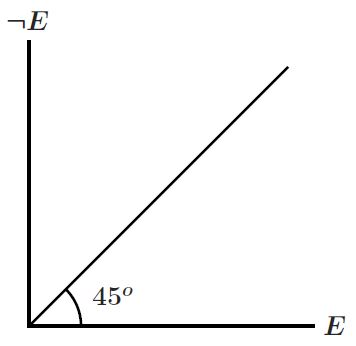
\includegraphics[scale=0.35]{images/certline}
\end{minipage} \hfill

\begin{remark}[Properties of $U(\cdot)$]
The utility function has some interesting properties on the graph:\begin{itemize}
\item Its MRS is given by: $$ -\frac{\partial U/\partial x}{\partial U/\partial y} = -\frac{p}{(1-p)}\frac{u'(x)}{u'(y)}$$
\item At the certainty line, we have that $x = y\Leftrightarrow u'(x) = u'(y)$, and thus the MRS is simply:$-\frac{p}{(1-p)}$. Note that this result is independent of $u(\cdot)$, meaning that it holds regardless of the utility curve used or the wealth level.
\item Being the sum of two concave function, $U(\cdot)$ is concave and hence quasi-concave.
\end{itemize}
\end{remark}

\begin{figure}[ht!]
\centering
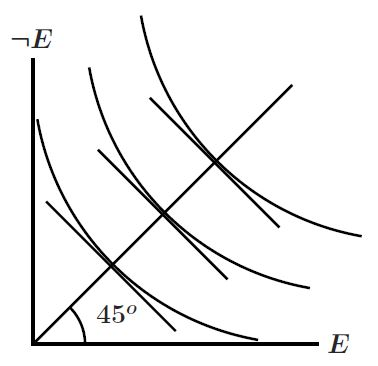
\includegraphics[scale=0.55]{images/mrsrisk}
\caption{Utility function representation on the plane}
\end{figure}

\subsection{Setting up the insurance problem}

Now we consider the decision-maker with wealth $w$. His wealth is subject to a risk of loss (the event $E$); in the case of $E$, the possible loss is $L$ which occurs with probability $p$ (the probability of accident). In order to escape the risk, he can choose to insure is assets. The price to fully insure one dollar of an asset is $q$. For example, if he choose to insure $Y$ (choice variable), it will cost him $qY$. 

If he buys $Y$ dollars of insurance, his new wealth is $w - qY$ and the individual will face the following risky situation:\begin{itemize}
\item In case of the bad event occurring, he loses $L$, and gets $Y$ back from the insurance company; his wealth is: $w - qY - L + Y$.
\item In case of the good event occurring, he doesn't lose anything and doesn't get any refund; his wealth is: $w - qY$.
\end{itemize}

Therefore, he faces the lottery $$ X = (w - qY - L + Y, p ; w - qY, (1-p)) $$ where he is able to choose the level of insurance $Y$. His expected utility is $$ U(X) = p\cdot u(w - qY - L + Y) + (1-p)\cdot u(w - qY)$$ The optimal level $Y^*$ should solve the following conditions:\begin{itemize}
\item FOC: $ (1-q)pu'(w - qY - L+Y) - q(1-p)u'(w - qY) = 0 $ $$\Leftrightarrow \frac{(1-q)}{q} = \frac{(1 - p)}{p}\frac{u'(w - qY)}{u'(w - qY - L + Y)} $$
\item SOC: $(1-q)^2pu''(w - qY - L+Y) + q^2(1-p)u''(w - qY) < 0 $ which will always be true due to the concavity of $u(\cdot)$.
\end{itemize}

As in a classic consumer problem, we also need to account for the budget constraint. Here, the equivalent to the budget constraint is the line of potential contracts under the price $q$.

\begin{minipage}{0.69\textwidth}
Graphically, no insurance would be the point $(w -L , w)$ while full insurance is $(w- qL, w-qL)$. Any partial insurance would be on the line between NI and FI (linear combination): this is the budget line! \\
$ \quad \Rightarrow$ its slope is $-q/(1-q)$.
\end{minipage}
\begin{minipage}{0.29\textwidth}
\centering
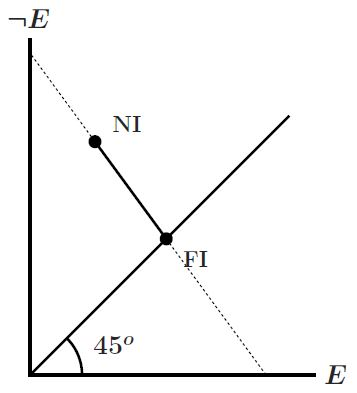
\includegraphics[scale=0.35]{images/budgline}
\end{minipage} \hfill

\begin{minipage}{0.69\textwidth}
Individuals will fully insure if the slope of their utility curve is steeper than the budget line, that is iff: $$ \frac{-pu'(w - qL)}{(1-p)u'(w - qL)} \leq -q/(1-q) \Leftrightarrow p\geq q$$ In words, this condition states that if the probability of loss is higher than the price of insurance, they will fully insure their assets.
\end{minipage}
\begin{minipage}{0.29\textwidth}
\centering
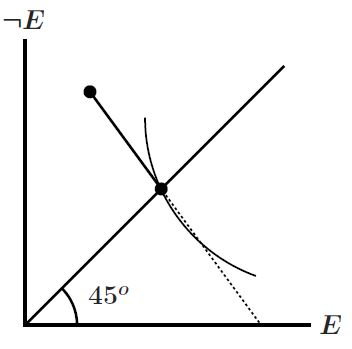
\includegraphics[scale=0.35]{images/fullins}
\end{minipage} \hfill

Note that these results hold if and only if the utilities are concave, meaning that the consumers are risk-averse.

Insurance companies will make profits if and only if $q \geq p$. Assuming a Bertrand competition setting, prices will have to go down to $q = p$; if not, some new insurance company could steal the profits by proposing a lower price.

Therefore in equilibrium, prices go to $p=q$ and everyone will buy full insurance.

\subsection{Different attitudes towards risk}

\subsubsection{Risk-neutrality}

Under risk-neutrality, we have that $u'(x) = u'(y)$ regardless of the values of $x$ and $y$. Thus we can write the first-order condition for buying insurance on $Y$ as: $$ \frac{(1-q)}{q} = \frac{(1 - p)}{p}\frac{u'(w - qY)}{u'(w - qY - L + Y)} $$ $$\Leftrightarrow \frac{(1-q)}{q} = \frac{(1 - p)}{p} $$ which is always true (regardless of the level of $Y$) is $q = p$. This means that when insurance companies price at $q = p$, a risk-neutral individual would buy any level of insurance.

If the price of insurance $q$ is strictly lower than $p$, then the slope of the budget line is less steep than the indifference curves of the individual: he buys full insurance.

If the price of insurance is $q > p$, then we are in the opposite situation, the risk-neutral individual buys no insurance.

This analysis reinforces the intuition behind risk-neutrality being an attitude that cares only about the monetary amount.   

\subsubsection{Risk-loving}

Under risk-loving preferences (convex utility) the decision of the agent is not obvious. The SOC conditions for sure do not hold, hence we are looking for a corner solution: a risk-loving individual will always choose full or no insurance. How do we know which contract the individual will choose? We cannot be sure always!

Remember that at the 45-degree line you have two important elements: the full-insurance contract (end of the budget line) and the MRS equal to $-p/(1-p)$. If, at this point, the budget line has a steeper slope than the MRS, this means that the individual can increase his utility by moving upwards the budget line: he will buy no insurance. This happens if: $$-\frac{q}{1-q} \leq -\frac{p}{1-p} \Leftrightarrow \frac{q}{1-q} \geq \frac{p}{1-p} \Leftrightarrow q\geq p$$ This result is the only certainty that we have about the behaviour of any risk-loving individual but it is of major importance. This implies that for any price higher than or equal to the probability of loss, a risk-loving individual will never choose to insure himself.

\section{Asymmetric information}

Now suppose there are two types of individuals:\begin{itemize}
\item $\lambda$ individuals with high risk of loss ($p_h$).
\item $(1-\lambda)$ individuals with low risk of loss ($p_l<p_h$).
\end{itemize}

\begin{minipage}{0.69\textwidth}
Let $A$ be the point of no insurance, it is the same point for both high and low risk types. For high risk types, full insurance will be at price $q_h = p_h$, call it point $B$. 
\end{minipage}
\begin{minipage}{0.29\textwidth}
\centering
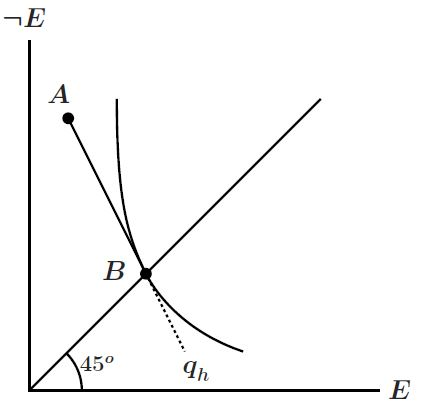
\includegraphics[scale=0.35]{images/hirisk}
\end{minipage} \hfill

\begin{minipage}{0.69\textwidth}
For low risk types, full insurance will be at price $q_l = p_l$, call it point $C$. Since $p_l < p_h$, the budget line for low risk types is less steep than for high risk, $C$ is higher than $B$ on the uncertainty line.
\end{minipage}
\begin{minipage}{0.29\textwidth}
\centering
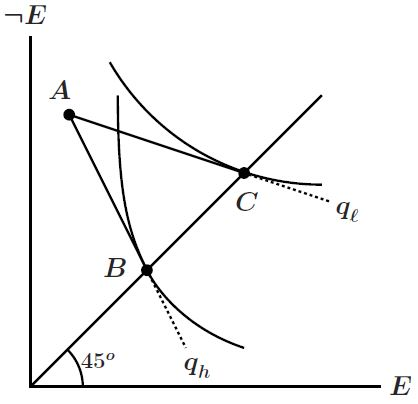
\includegraphics[scale=0.35]{images/lorisk}
\end{minipage} \hfill

Consider the setting where the type of an individual is privately known (the insurance firm does not know it), non-communicable and non-screenable. The insurance company has to design a contract to satisfy both consumers: is it possible?

\begin{minipage}{0.69\textwidth}
Let $q'$ be this contract price such that $q_h \geq q' \geq q_l$. 

Then high risk individuals will get full insurance at this price but for each one of them, the insurance company will make negative profits. They will choose point $D$.

Low risk individuals will certainly not fully insure their assets, however they might partially insure it: the insurance company may make positive profits. They will choose point $K$.
\end{minipage}
\begin{minipage}{0.29\textwidth}
\centering
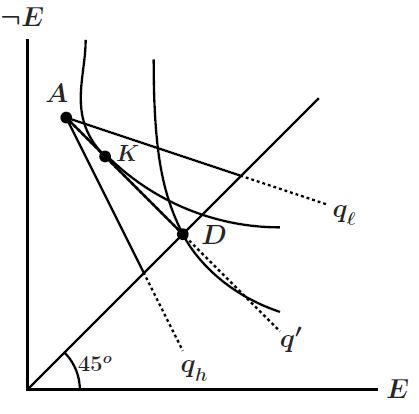
\includegraphics[scale=0.35]{images/advsel}
\end{minipage} \hfill

\begin{minipage}{0.69\textwidth}
In this situation, if the insurance company loses money it will not create any contract. If it makes zero profit, the situation is not stable as any point preferred to low-risk without being preferred to high-risk (e.g. point $F$) will make the market collapse. This is the issue of adverse selection.
\end{minipage}
\begin{minipage}{0.29\textwidth}
\centering
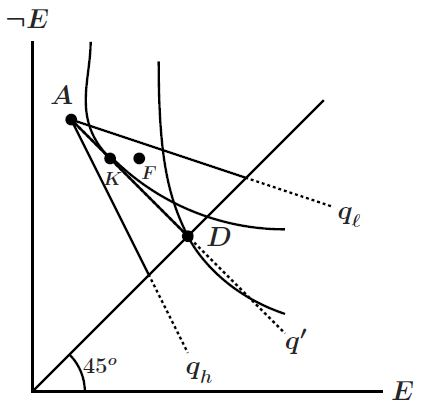
\includegraphics[scale=0.35]{images/advsel2}
\end{minipage} \hfill

One can think about two solutions:\begin{itemize}
\item Pooling contracts: these are one take-it-or-leave-it options such that high and low risk individuals have to get this unique contract or not be insured.
\item Separating contracts: two contracts such that no type has an incentive to get the other contract.
\end{itemize}

\chapter{Stochastic dominance}

This chapter tries to answer the question of determining the best lotteries among different lotteries. For example, let two lotteries be $X = (150, H; 70, T)$ and $Y=(60,H;120,T)$, how can we determine the best lottery (analytically)?

\begin{definition}
Let X be any lottery. The cumulative distribution function (or cdf) of the lottery $X$ is the function $F_X$ such that, $$F_X(x) = \Prob{X\leq x} $$
\end{definition}

\begin{definition}[First-Order Stochastic Dominance]
Let $X$ and $Y$ be any two lotteries with cdf $F_X$ and $F_Y$ resp. We say that $X$ dominates $Y$ by FOSD if and only if, for all $x$, $$F_X(x) \leq F_Y(x) \Leftrightarrow  \Prob{X\leq x} \leq \Prob{Y\leq x} $$
\end{definition}

\begin{figure}[ht!]
\centering
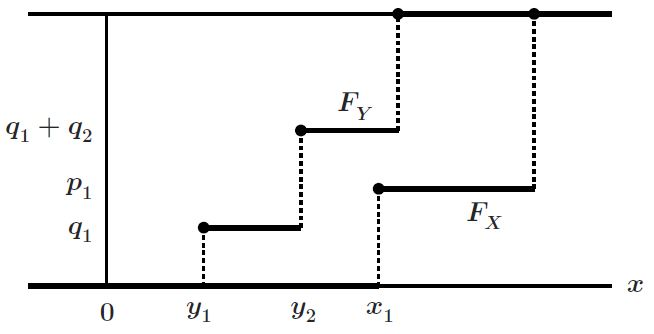
\includegraphics[scale=0.45]{images/fosd}
\end{figure}

\begin{definition}
We say that a preference relation $\succeq$ satisfy the FOSD axiom if, $$X\succeq Y \Leftrightarrow X\text{ dominates } Y \text{ by FOSD.} $$
\end{definition}

\begin{remark}
Let $X$ and $Y$ be two lotteries such that,\begin{itemize}
\item $X = (x_1, p_1; ... ; x_n, p_n)$
\item $Y = (y_1, p_1; ... ; y_n, p_n)$
\end{itemize} If for all $i$, $x_i \geq y_i$, then $X$ dominates $Y$ by FOSD.
\end{remark}

\begin{proof}
For all $x$, define two functions:\begin{itemize}
\item $I_X(x) = \left\lbrace i: x_i\leq x\right\rbrace$
\item $I_Y(x) = \left\lbrace i: y_i\leq x\right\rbrace$
\end{itemize}
By assumption, for any $x$, $I_X(x)\subseteq I_Y(x)$. Now, $$F_X(x) = \sum_{i\in I_X(x)} p_i \leq \sum_{i\in I_Y(x)} p_i = F_Y(x) $$ which by definition 5.2, implies that $X$ dominates $Y$ by FOSD.
\end{proof}

\begin{remark}
Let $X$ and $Y$ be two finite lotteries such that $X$ dominates $Y$ by FOSD, then there exists an alternative notation $$ X = (x_1', r_1; ...; x_n', r_n) \textit{ and }Y = (y_1', r_1; ...; y_n', r_n)$$ such that $x_1' \geq y_1'$ for all $i$.
\end{remark}

\begin{bclogo}[couleur=blue!10, arrondi=0.1, logo=,ombre=false]{ First-Order Stochastic Dominance: an example} 
\begin{small}
Let $X$ and $Y$ be two lotteries defined as: \begin{itemize}
\item $X = \left(100, \frac{1}{2}; 50, \frac{1}{4} ; 20, \frac{1}{4}\right)$
\item $Y = \left(70, \frac{1}{3};50, \frac{1}{3}; 10, \frac{1}{3}\right)$
\end{itemize}
We can rewrite them as: $$X = \left(100, \frac{1}{3}; 100, \frac{1}{6}; 50, \frac{1}{6} ; 50, \frac{1}{12} ; 20, \frac{1}{4}\right)$$ and 
$$ Y = \left(70, \frac{1}{3};50, \frac{1}{6};50, \frac{1}{6}; 10, \frac{1}{12}; 10, \frac{1}{4}\right)$$ which makes it clear that $X$ dominates $Y$ by FOSD.
\end{small}
\end{bclogo}

\begin{theorem}
Let $X$ and $Y$ be two lotteries and $u(\cdot)$ an increasing utility function. $X$ dominates $Y$ by FOSD if and only if, $\E{u(X)} \geq	\E{u(Y)}$.
\end{theorem}

\begin{proof}
($\Rightarrow$): Let $X$ dominate $Y$ by FOSD. From the previous remark, we can write the two lotteries as $$X=(x_1, r_1; ...; x_n, r_n) \textit{ and } Y = (y_1, r_1; ...; y_n, r_n) $$ where $x_i \geq y_i$ for all i. Using th efact that $u(\cdot)$ is increasing, we have $u(x_i)\geq u(y_i)$ and hence $$\E{u(X)} \geq \E{u(Y)}$$ ($\Leftarrow$): the rest of the proof will be shown by intuition with examples showing by contraposition that non-dominance will imply that $u(\cdot)$ is not increasing.
\end{proof}

\begin{definition}
Suppose all outcomes of two lotteries $X$ and $Y$ fall in the set $\left[a, b\right]$. Then, $X$ dominates $Y$ by Second-Order Stochastic Dominance (SOSD) if for all $x$, $$\int_a^x F_X(z)\D z \leq \int_a^x F_Y(z)\D z $$ and $$\int_a^b F_X(z)\D z = \int_a^b F_Y(z)\D z $$ This means that while $\E{X} = \E{Y}$, $X$ gives a higher probability to win more than $x$ for all $x$.
\end{definition}

\begin{figure}[ht!]
\centering
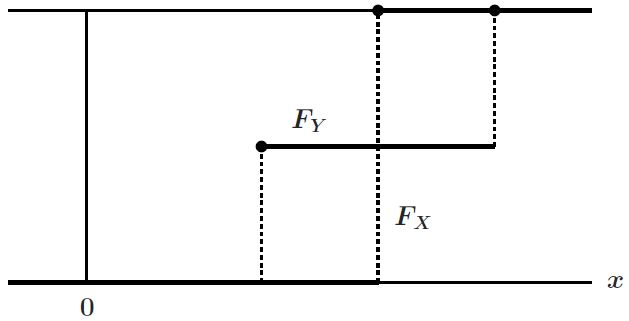
\includegraphics[scale=0.33]{images/sosd}
\end{figure}

\begin{bclogo}[couleur=blue!10, arrondi=0.1, logo=,ombre=false]{ Second-Order Stochastic Dominance: an example} 
\begin{small}
Let $X$ and $Y$ be two lotteries defined as: \begin{itemize}
\item $X = \left(-100, \frac{1}{2}; 100, \frac{1}{2}\right)$
\item $Y = \left(-100, \frac{1}{4}; 0, \frac{1}{2}; 100, \frac{1}{4}\right)$
\end{itemize}
Here, $Y$ dominates $X$ by FOSD.
\end{small}
\end{bclogo}

\begin{theorem}
Let $X$ and $Y$ be two lotteries such that $\E{X} = \E{Y}$ and $u(\cdot)$ an increasing utility function. $X$ dominates $Y$ by SOSD if and only if, $\E{u(X)} \geq	\E{u(Y)}$.
\end{theorem}

\chapter{Alternatives to EU theory}

\section{Allais Paradox}

Consider two lotteries $A$ and $B$ such that:\begin{itemize}
\item $A = (5M, 0.1; 0, 0.9)$
\item $B = (1M, 0.11; 0, 0.89)$
\end{itemize}
Usually people prefer lottery $A$.

Now, let's study:\begin{itemize}
\item $C = (5M, 0.1; 1M, 0.89; 0, 0.01)$
\item $D = (1M, 1)$
\end{itemize}
Then people prefer $D$ to $C$.

However, by EU:\begin{align*}
A\succeq B \Leftrightarrow 0.1u(5M) \geq 0.11u(1M) & \Leftrightarrow 0.1u(5M) + 0.89(1M) \geq u(1M) \\ & \Leftrightarrow C\succeq D
\end{align*}
This is called the Allais paradox.

\section{Common Ratio Effect}

Consider two lotteries $A$ and $B$ such that:\begin{itemize}
\item $A = (3000, 1)$
\item $B = (4000, 0.8; 0, 0.2)$
\end{itemize}
Usually people prefer lottery $A$.

Now, let's study:\begin{itemize}
\item $C = (3000, 0.25; 0, 0.75)$
\item $D = (4000, 0.2; 0.8)$
\end{itemize}
Then people prefer $D$ to $C$.

However, by EU:\begin{align*}
A\succeq B \Leftrightarrow u(3000) \geq 0.8u(4000) & \Leftrightarrow 0.25u(3000) \geq 0.2u(4000) \\ & \Leftrightarrow C\succeq D
\end{align*}
This is called the Common Ratio Effect.

\section{Sure Thing Principle}

The Sure Thing Principle, introduced by Savage (1972) is linked to the independence axiom. In particular, it states that if an event does not happen, then the outcomes associated to it should not matter. Formally, let $f, g, f'$ and $g'$ be outcomes related to the event $E$.

When $E$ happens, then outcomes $f = f'$ and $g=g'$; when $\neg E$ happens, $f = g$ and $f' = g'$. If an individual has preferences $f\succeq g$, then $f'\succeq g'$.

This theory can be close to EU theory as it ignores the psychological effect of changing the menu: here what happens to $\neg E$.

\begin{bclogo}[couleur=blue!10, arrondi=0.1, logo=,ombre=false]{ The STP applied to Allais' paradox} 
\begin{small}
Define outcomes of $A, B, C$ and $D$ in the same manner as in the Allais paradox lotteries. Define event $E$ such that it is equivalent to drawing any ball between $1$ and $11$, while $\neg E$ would be the balls numbered $12$ to $100$.

Then the outcomes of $A$ and $C$ are the same under $E$ but differ under $\neg E$. The same comparison goes for $B$ and $D$. If $A\succeq B$, then $C\succeq D$ because there is no change between the two elements within the pairs relative to the outcomes in $\neg E$.

The conclusion is the same as in EU theory, hence it also creates the Allais paradox.
\end{small}
\end{bclogo}

\section{Prospect Theory}

Prospect theory, introduced by Kahneman and Tversky tries to solve the Allais paradox issue by stating that people have biases in how to analyze probabilities. In particular, the define a function $\pi(p)$ that relates actual probabilities to what individuals consider as probabilities. The formulation is the same as in the EU theory with different probabilities:$$V = \sum\pi(p_i)u(x_i)$$ where $\pi(p_i)$ is the probability weighting function allowing people to react differently to probability changes.

\begin{bclogo}[couleur=blue!10, arrondi=0.1, logo=,ombre=false]{ Prospect Theory applied to the Common Ratio Effect} 
\begin{small}
Let $u(x) = x$ for simplicity. Define $\pi(0.8) = 0.7$, $\pi(0.25) = 0.25$ and $\pi(0.2) = 0.2$. Then,\begin{itemize}
\item $V((3000,1)) = 3000$
\item $V((4000, 0.8;0,0.2)) = 2800$
\item $V((3000, 0.25;0,0.75)) = 750$
\item $V((4000, 0.2; 0, 0.8)) = 800$
\end{itemize}
And you have rationalized that $A\succeq B$ but $D\succeq C$.
\end{small}
\end{bclogo}

\subsection{Issues with prospect theory}

There are some issues relating to the probability weighting function considered in the probability theory.

Let there be two lotteries:$$(x, p+q; 0, 1-p-q) \sim (x,p;x,q;0,1-p-q)$$ The equivalence between the two lotteries is obvious, but leads to the necessity of $\pi(p+q) = \pi(p) + \pi(q)$. This implies necessarily that $\pi(p) = p$.

Kahneman and Tversky address the issue by saying that obvious comparisons between lotteries cannot be included in prospect theory.

We could for example use FOSD to justify that those two lotteries are equivalent.

However, let $\varepsilon_n$ be such that:$$(x + \frac{1}{n}, p; x-\varepsilon_n, q; 0, 1-p-q) \sim (x, p+q; 0, 1-p-q)$$ This implies that $$u(x+\frac{1}{n})\pi(p) + u(x-\varepsilon_n)\pi(q) = u(x)\pi(p+q) $$ When $n\to\infty$, then $1/n\to 0$ and consequently $\varepsilon_n\to 0$. Hence we get again:$$\pi(p)+\pi(q) = \pi(p+q)$$

\section{Rank Dependent Probabilities}

This theory was brought up by Quiggin (1982). For an ordered lottery $X = (x_1, p_1; ...;x_n, p_n)$, consider$$V(X) = u(x_1)f(p_1) + \sum_{i=2}^{n}u(x_i)\left[f\left(\sum_{j=1}^{i}p_i \right)-f\left(\sum_{j=1}^{i-1}p_i\right)\right] $$ In the case where $f(p) = p$, we have EU theory.

In particular, in a two-state lottery of the form $X=(x,p;y,1-p)$, we get:\begin{align*}
V(X) = \begin{cases}
u(x)f(p) + u(y)[1 - f(p)] & \text{if } x\leq y \\
u(x)[1-f(1-p)] + u(y)f(1-p) & \text{if } x > y
\end{cases}
\end{align*}

\begin{bclogo}[couleur=blue!10, arrondi=0.1, logo=,ombre=false]{ Rank Dependent probabilities applied to the Common Ratio Effect} 
\begin{small}
In the CRE, we have:\begin{itemize}
\item $V((3000,1)) = u(3000)$
\item $V((4000, 0.8;0,0.2)) = u(4000)[1 - f(0.2)]$
\item $V((3000, 0.25;0,0.75)) = u(3000)[1-f(0.75)]$
\item $V((4000, 0.2; 0, 0.8)) = u(4000)[1-f(0.8)]$
\end{itemize}
Hence, $$A\succeq B \Leftrightarrow u(3000) \geq u(4000)[1-f(0.2)] \Leftrightarrow \frac{u(3000)}{u(4000)} \geq 1 - f(0.2) $$
Meanwhile, $$D\succeq C \Leftrightarrow u(4000)[1-f(0.8)]\geq u(3000)[1-f(0.75)] \Leftrightarrow \frac{1-f(0.8)}{1-f(0.75)} \geq \frac{u(3000)}{u(4000)} $$ which in the end gives: $$ 1 - f(0.2)\leq\frac{u(3000)}{u(4000)} \leq \frac{1-f(0.8)}{1-f(0.75)} $$ You can verify that it holds for $f(p) = \sqrt{p}$ and $u(x) = x$.
\end{small}
\end{bclogo}

Now, we might ask how this utility form applies to the space of lotteries. We have:\begin{align*}MRS^{xy} = 
\begin{cases}
-\frac{u'(x)f(p)}{u'(y)[1 - f(p)]} & \text{if } x<y\\
-\frac{f(p)}{1-f(p)} & \text{if } x\to y\\
-\frac{1-f(p)}{f(p)} & \text{if } y\to x\\
-\frac{u'(x)[1-f(1-p)]}{u'(y)f(1-p)} & \text{if } x>y\\
\end{cases}
\end{align*}
which graphically gives a kink on the certainty line: \begin{figure}[ht!]
\centering
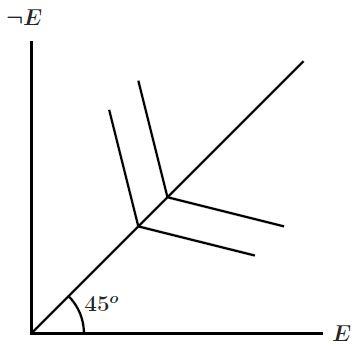
\includegraphics[scale=0.6]{images/rdprob}
\end{figure}

Because of the fact that the slope of the indifference curves are constant, even if the price of insurance is higher than the probability of loss, you get an individual who'd be willing to fully insure.
\begin{figure}[ht!]
\centering
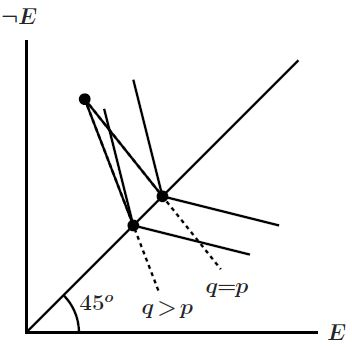
\includegraphics[scale=0.6]{images/rdprobfi}
\end{figure}

\section{Marschak-Machina Probability Triangle}

Machina (1982) provided a new insight in this set of problems in which you could remap the lottery space in a probability space.

Consider $x>y>z$ and consider the set:$$\{(p,q)\in\mathbb{R}_+^2 : p+q\leq 1\} $$

The lottery $X = (x, p; y, 1-p-q; z, q)$ could be represented in this space by defining $p$ as its ordinate and $q$ its absciss.
\begin{figure}[ht!]
\centering
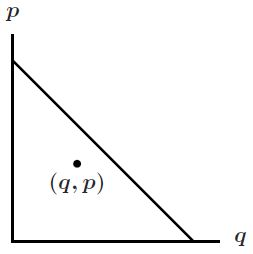
\includegraphics[scale=0.7]{images/machinatri}
\end{figure}

The EU of this lottery is: $$\operatorname{EU}(X) = pu(x) + (1-p-q)u(y) + qu(z)$$ Maximizing this utility function gives:\begin{itemize}
\item $\frac{\partial \operatorname{EU}(X)}{\partial p} = 0 \Leftrightarrow u(x) - u(y)$
\item $\frac{\partial \operatorname{EU}(X)}{\partial q} = 0 \Leftrightarrow -u(y) + u(z)$
\end{itemize}
Which gives the following $$\operatorname{MRS}^{pq} = -\frac{u(z) - u(y)}{u(x) - u(y)} = \frac{u(y) - u(z)}{u(x) - u(y)} $$ which gives constant slopes to the indifference curves of $\operatorname{EU}(X)$ over the space of probabilities.

\subsection{Machina triangle applied to the Allais paradox}
Define $x = 5M, y =1M, z = 0$, and pairs $(p,q)$ such that:\begin{itemize}
\item $A = (0.1,0.9)$
\item $B = (0, 0.89)$
\item $C = (0.1, 0.01)$
\item $D = (0,0)$
\end{itemize}
Then, graphically we obtain:
\begin{figure}[ht!]
\centering
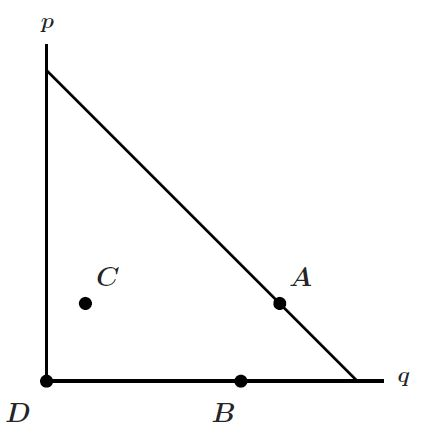
\includegraphics[scale=0.43]{images/machinaallais}
\end{figure}

With parallel indifference curves, we want to find a match where $A\succ B$ but $D\succ C$:
\begin{figure}[ht!]
\centering
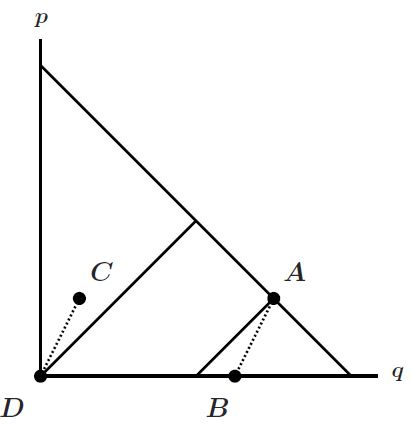
\includegraphics[scale=0.43]{images/machinaallais2}
\end{figure}

However, this is only possible if the lines change slopes as in:
\begin{figure}[ht!]
\centering
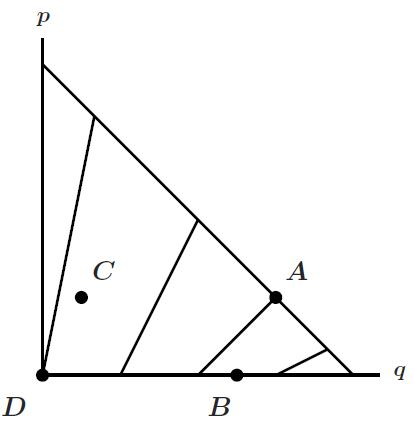
\includegraphics[scale=0.43]{images/machinaallais3}
\end{figure}

This issue can not be reconciled with differentiable equations as in EU theory. However, some fonctional forms exist that satisfy Machina's structure.

For example, $$V(X) = \E{u(X)}^2 + \E{v(X)}$$ where $u$ and $v$ are not linear transformations of each other. Or, $$V(X) = \frac{\E{u(X)}}{\E{v(X)}}$$

\chapter{Preference reversals and violations of transitivity}

\section{Violations of transitivity}

Lichtenstein and Slovic (1971) designed the following experiment: let $P=(4,\frac{35}{36};-1,\frac{1}{36})$ and $S = (16, \frac{11}{36}; -1.5, \frac{25}{36})$. While the expected value of $P$ is higher than of $S$, people prefer $P$ to $S$.


\end{document}